\documentclass{tufte-handout}

\title{GGSB 2015 Prelim} %\thanks{Inspired by Edward~R. Tufte!}}

\author[The Tufte-LaTeX Developers]{Charles Czysz}

\date{September 2015} % without \date command, current date is supplied

\setcounter{tocdepth}{3}

%\geometry{showframe} % display margins for debugging page layout

\usepackage{hyperref}
\hypersetup{
  colorlinks   = true,    % Colours links instead of ugly boxes
  urlcolor     = blue,    % Colour for external hyperlinks
  linkcolor    = black,    % Colour of internal links
  citecolor    = red      % Colour of citations
}
\usepackage{graphicx} % allow embedded images
  %\setkeys{Gin}{width=\linewidth,totalheight=\textheight,keepaspectratio}
  \graphicspath{{./figs}} % set of paths to search for images
\usepackage{amsmath}  % extended mathematics
\usepackage{booktabs} % book-quality tables
\usepackage{units}    % non-stacked fractions and better unit spacing
\usepackage{multicol} % multiple column layout facilities
\usepackage{lipsum}   % filler text
\usepackage{fancyvrb} % extended verbatim environments
\usepackage{amsthm}
  \fvset{fontsize=\normalsize}% default font size for fancy-verbatim environments

% Standardize command font styles and environments
\newcommand{\doccmd}[1]{\texttt{\textbackslash#1}}% command name -- adds backslash automatically
\newcommand{\docopt}[1]{\ensuremath{\langle}\textrm{\textit{#1}}\ensuremath{\rangle}}% optional command argument
\newcommand{\docarg}[1]{\textrm{\textit{#1}}}% (required) command argument
\newcommand{\docenv}[1]{\textsf{#1}}% environment name
\newcommand{\docpkg}[1]{\texttt{#1}}% package name
\newcommand{\doccls}[1]{\texttt{#1}}% document class name
\newcommand{\docclsopt}[1]{\texttt{#1}}% document class option name
\newenvironment{docspec}{\begin{quote}\noindent}{\end{quote}}% command specification environment

\newtheorem*{define}{Definition}

% Normal font formatting for subsections (i.e. questions)
\titleformat{\subsection}
{\large\bfseries}{\thesection}{1em}{}
%\normalfont
\usepackage{makeidx}
\makeindex


\begin{document}

\maketitle% this prints the handout title, author, and date

\noindent
\textbf{Required}

Questions 1-8: General Genetic Principles

Questions 9-12: Mapping

Questions 39-50: Study Design and Statistical Data Analysis

\vspace*{1\baselineskip}

\noindent
\textbf{Choice between}

Questions 13-17: Genetic Architecture of Human Phenotypes

\textbf{or}

Questions 18-28: Population and Evolutionary Genetics

\vspace*{1\baselineskip}

Questions 29-32: Molecular Mechanisms and Model Organisms in Human Genetics

\textbf{or}

Questions 33-38: Gene Regulation and Human Phenotypes

\vspace*{4\baselineskip}
\begin{abstract}
\noindent
A good answer would show in escalating order: 
\begin{itemize}
\item Basic understanding via descriptions and definition of basic terms and concepts 
\item Knowledge of biology/literature via empirical examples of concepts in action, 
\item Engagement of critical thinking by highlighting well-known limitations or novel critiques of a concept or its common application 
\item Recognition of open problems and novel research opportunities.
\end{itemize}

\end{abstract}

\newpage

\tableofcontents 

\newpage
%\printclassoptions
 
\section{General Genetic Principles}\label{sec:gen-genetic}

\subsection{1.
Explain the distinction between allelic heterogeneity, genetic (locus) heterogeneity, and clinical heterogeneity. Give examples of each.}  
%\label{subsec:01}

\begin{abstract}
Great review of this topic:

\href{http://www.sciencedirect.com/science/article/pii/S009286741000320X}{Genetic Heterogeneity in Human Diseases}
\end{abstract}
%This question asks to explain how similar or identical phenotypes can have different underlying causes.

\noindent
\textbf{Overview}

\noindent
Each of the following topics have implications in the type of studies which can or cannot be used. Overall, heterogeneity ensures that large-scale association tests or case-control studies will be poorly powered to detect causal variants or genes. See the review linked above for more detail.

%\define[Allelic heterogeneity]
\begin{define}[Allelic Heterogeneity]
In a given population, different mutations in the same gene result in a similar phenotype.
\end{define}
\noindent
\textbf{Example} 

Cystic Fibrosis is caused by defective cystic fibrosis transmembrane conductance regulator proteins (CFTR). Many mutations in the CFTR gene can give rise to non-functioning proteins, which all lead to the same CF phenotype.

Two-thirds of all CF mutations are a 3bp deletion at position 508, resulting in a loss of phenylalanine. 1,500 other mutations also exist which lead to CF. However, this disease is haplosufficient..

Unknown alleleic heterogeneity can affect GWA results\footnote{\url{http://hmg.oxfordjournals.org/content/11/20/2417.short}} when LD methods are used.

\textbf{Sources}

\url{http://hmg.oxfordjournals.org/content/20/20/4082.short}

\begin{define}[Genetic (locus) heterogeneity]
Mutations in different genes result in a similar phenotype.
\end{define}

The BRCA1 and BRCA2 genes are a good example of how mutations in different genes lead to the same phenotype. 

\begin{define}[Clinical Heterogeneity]
Variability in clinical manifestations, or phenotypes, with the same underlying mutation/genetic disorder.
\end{define}

\newpage
Mutations in several genes can lead to familial hypercholesterolemia, high level of LDL cholesterol. Mutations in LDLR (LDL receptor), Apolipoprotein B, proprotein convertase subtilisin/kexin type 9 (PCSK9), and the ARH/LDLRAP1 genes can all lead to familial hypercholesterolemia.
\subsection{2.
What is the relationship between the inbreeding coefficient, kinship coefficient, and coefficient of relatedness? How are they calculated in pedigrees? Can they be estimated in the absence of pedigree information?}
\label{subsec:02} 

\begin{define}[Identity by descent]
Two alleles at the same locus that are descended from the same ancestral allele within the recent past.
\end{define}

\begin{marginfigure}%
  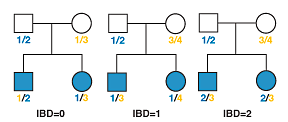
\includegraphics[scale=0.65]{./figs/ibd}
  \caption{IBD Pedigree Example}
  \label{fig:marginfig}
\end{marginfigure}

\begin{define}[Coefficient of Kinship]
$f_{xy}$: The probability that two alleles, one from X and the other from Y, are IBD.
\end{define}

\begin{figure}
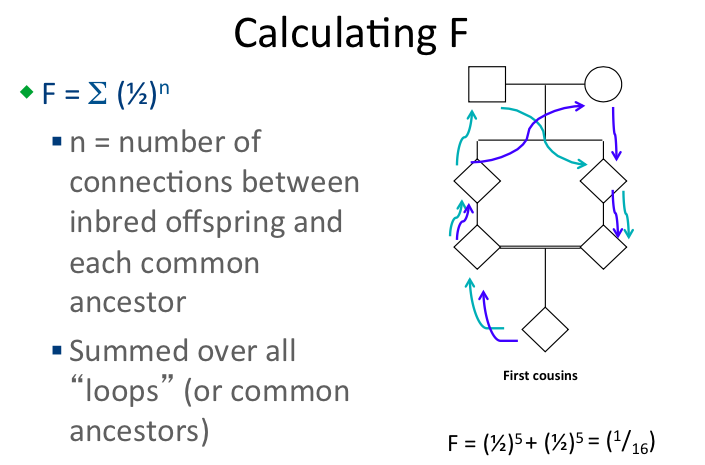
\includegraphics[scale=0.5]{./figs/kincoeff}
\end{figure}

\begin{define}[Coefficient of Relatedness]
$R_n$, the probability of sharing $n \in \{0,1,2\}$ IBD alleles. Mean relatedness, $\bar{r} = r_1 + 2r_2$.
\end{define}

\noindent
\textbf{Relationship between Coefficients}
\[f_{xy} = \frac{1}{2}\bar{r}\]
\begin{figure}
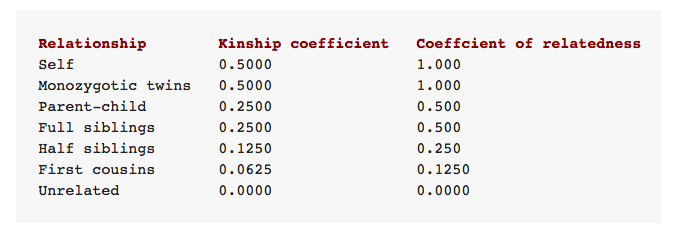
\includegraphics[scale=0.5]{./figs/kinrelate}
\caption{Relationship between Kinship and Relatedness coefficients}
\end{figure}


\newpage
\subsection{3.
What are the key distinguishing characteristics of pedigrees segregating autosomal dominant, autosomal recessive, X-linked, Y-linked, and mitochondrial diseases?}
\label{subsec:03}

\subsection{4.
Explain the "non-Mendelian" concepts of uniparental disomy and imprinting. How would these be manifested in pedigrees and how are they demonstrated at the cellular or molecular levels?}
\label{subsec:04}

\subsection{5.
What evidence is there for the presence of modifier loci? How is this related to the concept of epistasis and how is it distinct (or not) from polygenic and other models of inheritance?}
\label{subsec:05}

\subsection{6.
What are distinctions among the concepts linkage, linkage disequilibrium, and association? Under what circumstances would each be preferable for genetic mapping? Consider both sample composition and types of diseases.}
\label{subsec:06}

\subsection{7.
Define epistasis. Describe approaches that allow epistasis to be detected or quantified. Describe some biological mechanisms that can produce epistasis. Discuss the implications of epistasis for efforts to map the genetic causes of phenotypes. Discuss the potential implications of epistasis for the evolutionary process.}
\label{subsec:07}

\subsection{8.
Define heritability. Describe methods used to quantify the heritability of a phenotype. Discuss the value and limitations of heritability as a descriptor of the extent to which a phenotype has genetic causes. Describe the "missing heritability problem" and its potential explanations.}
\label{subsec:08}

\section{Mapping}\label{sec:map}
\end{document}
